\Chapter{Ütközések számítása}

A háromszöget metszéspontjának számításához elsősorban szükségünk van 2 háromszögre, mint input. Ezek lesznek az $\textbf{A}_0$, $\textbf{A}_1$, $\textbf{A}_2$, illetve $\textbf{B}_0$, $\textbf{B}_1$, $\textbf{B}_2$ csúcspontjaink. A csúcspontok segítségével kiszámíthatjuk a háromszögek éleit. Ezek lesznek az $\textbf{C}_0$, $\textbf{C}_1$, $\textbf{C}_2$, illetve $\textbf{E}_0$, $\textbf{E}_1$, $\textbf{E}_2$ élek. \\
$$\textbf{C}_0 = \textbf{A}_1 - \textbf{A}_0, \textbf{C}_1 = \textbf{A}_2 - \textbf{A}_0, \textbf{C}_2 = \textbf{C}_1 - \textbf{C}_0$$\\
Az élek segítségével kiszámíthatjuk a háromszögek normál vektorait. Ezek lesznek a \textbf{D}, illetve \textbf{F} vektorok.  \\
$$\textbf{D = C}_0 \times \textbf{C}_1$$\\
A számítások megkönnyítéséhez kiszámítjuk az eltolásvektort is.  \\
$$\textbf{G = B}_0 -\textbf{A}_0$$\\
Ezen adatok szolgálják a program számára az alapokat, amelyekből további számításokat végzünk. A metszés eldöntéséhez a következő univerzális képletet használjuk: 
$$\textbf{H}_1 = \textbf{L * C}_0$$
$$\textbf{H}_2 = \textbf{L * C}_1$$
$$\textbf{I}_0 = \textbf{L * G}$$
$$\textbf{I}_1 = \textbf{I}_0 + \textbf{L * E}_0$$
$$\textbf{I}_2 =\textbf{ I}_0 + \textbf{L * E}_1$$
\\
Minden sor 1-1 számítást jelent. Minden számítás után ellenőriznünk kell, hogy a két adott háromszög metszi-e egymást, vagy sem. Erre a következő képletet használjuk: Ha\\
$$\textbf{min(H) > max(I) vagy max(H) < min(I)}$$, akkor a két háromszögre biztosan mondható, hogy nem metszik egymást. Ez esetben nem szükséges további számításokat végezni. Amennyiben nemleges választ kapunk, akkor tovább kell számítanunk minden sort. Ha az utolsó sor esetén sem kapunk pozitív választ, akkor kimondhatjuk, hogy a két háromszög metszi egymást.

\newpage
\begin{table}[h]
	\centering
	\caption{A számítások táblázata.}
	\begin{tabular}{|c||c|c|c|c|c|}
		\hline
		\textbf{L}     & $\textbf{H}_1$   & $\textbf{H}_2$    & $\textbf{I}_0$      & $\textbf{I}_1$        & $\textbf{I}_2$        \\ \hline
		\textbf{D}     & 0    & 0     & D*G     & I0 + D*$E_0$ & I0 + D*$E_1$ \\ \hline
		\textbf{F}     & F*$C_0$ & F*$C_1$  & F*G     & $I_0$        & $I_0$        \\ \hline
		$\textbf{C}_0$*$\textbf{E}_0$ & 0    & -D*$E_0$ & $C_0$x$E_0$*G & $I_0$        & $I_0$ + F*$C_0$ \\ \hline
		$\textbf{C}_0$*$\textbf{E}_1$ & 0    & -D*$E_1$ & $C_0$x$E_1$*G & $I_0$ - F*$C_0$ & $I_0$        \\ \hline
		$\textbf{C}_0$*$\textbf{E}_2$ & 0    & -D*$E_2$ & $C_0$x$E_2$*G & $I_0$ - F*$C_0$ & $I_1$        \\ \hline
		$\textbf{C}_1$*$\textbf{E}_0$ & D*$E_0$ & 0     & $C_1$x$E_0$*G & $I_0$        & $I_0$ + F*$C_1$ \\ \hline
		$\textbf{C}_1$*$\textbf{E}_1$ & D*$E_1$ & 0     & $C_1$x$E_1$*G & $I_0$ - F*$C_1$ & $I_0$        \\ \hline
		$\textbf{C}_1$*$\textbf{E}_2$ & D*$E_2$ & 0     & $C_1$x$E_2$*G & $I_0$ - F*$C_1$ & $I_1$        \\ \hline
		$\textbf{C}_2$*$\textbf{E}_0$ & D*$E_0$ & $H_1$    & $C_2$x$E_0$*G & $I_0$        & $I_0$ + F*$C_2$ \\ \hline
		$\textbf{C}_2$*$\textbf{E}_1$ & D*$E_1$ & $H_1$    & $C_2$x$E_1$*G & $I_0$ - F*$C_2$ & $I_0$        \\ \hline
		$\textbf{C}_2$*$\textbf{E}_2$ & D*$E_2$ & $H_1$   & $C_2$x$E_2$*G & $I_0$ - F*$C_2$ & $I_1$        \\ \hline
	\end{tabular}
\end{table}
\newpage

\Section{Függvények kapcsolata}


\begin{figure}[h]
	\centering
	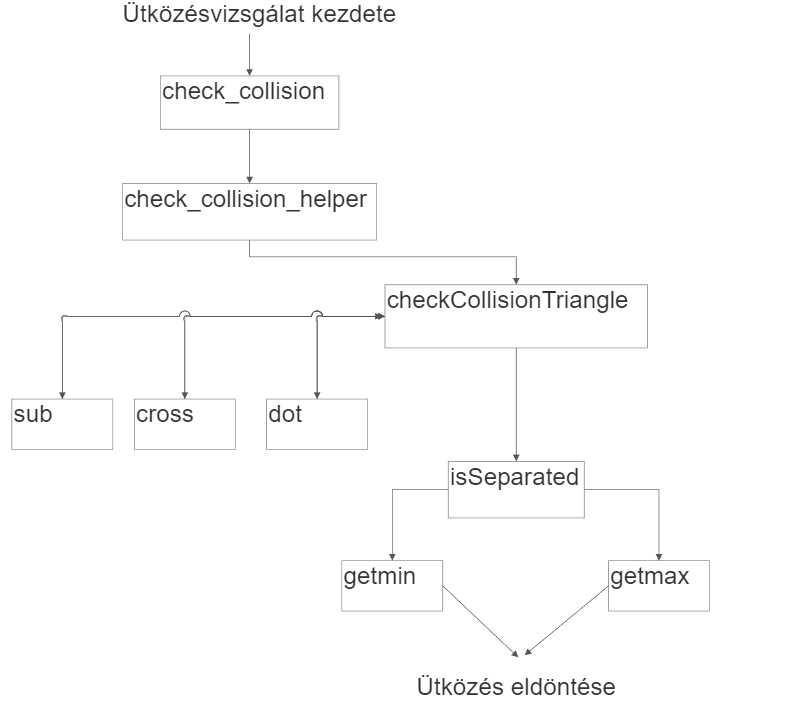
\includegraphics[width=15truecm, height=15truecm]{images/blokk_diagram.png}
	\caption{Függvénykönyvtár blokk diagramja}
	\label{fig:blokkdiagram}
\end{figure}


\newpage
